% ---------------------------------------------------------------
% Results section. Preamble requirements:
%   \usepackage{booktabs}
%   \usepackage{graphicx}
% For Calibri body text, compile with XeLaTeX or LuaLaTeX and add:
%   \usepackage{fontspec}
%   \setmainfont{Calibri}          % or \setmainfont{Carlito} on Linux
% (The figures are already set in Calibri/Carlito.)
% Figures expected in the same directory as this file:
%   ruminant_pop.png  ruminant_prod.png  ruminant_feed.png
%   nonrum_pop.png    nonrum_prod.png    nonrum_feed.png
% ---------------------------------------------------------------

\section{Results and Discussion}

Population and production are reported over 2019--2041. The 2019 values are
historical observations; 2020--2041 are model projections. The 2019 baseline is
therefore shown shaded in the figures, with the 2019--2020 segment drawn dotted,
and where the transition from historical to projected data produces a step
(Section~\ref{sec:dq}) growth rates are quoted from 2020. Feed demand carries no 2019
historical value and is reported over 2020--2041 throughout. 

\subsection{Population}

\subsubsection{Ruminants}

Total ruminant numbers rise from 88.0 million head in 2019 to 272.1 million in
2041, a 3.1-fold increase equivalent to 5.3\,\% per year (Table~\ref{tab:rumpop},
Figure~\ref{fig:rumpop}). Growth is not evenly distributed across value chains. Beef cattle expand
fastest at 6.6\,\% per year, quadrupling to 67.8 million head and overtaking
sheep as the second-largest ruminant population in 2036. Goats remain the
largest single population throughout, growing 5.9\,\% per year to 121.3 million.
Camels and dairy cattle follow intermediate trajectories of 5.2\,\% and
4.9\,\% per year respectively, each roughly tripling. Sheep are the
slowest-growing ruminant chain at 3.3\,\% per year, doubling over the period;
their share of the ruminant herd falls from 31.2\,\% in 2019 to
20.5\,\% in 2041.

\begin{table}[htbp]
\centering
\caption{Ruminant population, 2019--2041 (thousand head)}
\label{tab:rumpop}
\small
\begin{tabular}{lrrrrrr}
\toprule
\textbf{Series} (\,000 head) & \textbf{2019} & \textbf{2025} & \textbf{2030} & \textbf{2035} & \textbf{2041} & \textbf{CAGR 2019--41 (\%)} \\
\midrule
Goats & 34\,658 & 50\,854 & 66\,733 & 87\,571 & 121\,333 & 5.9 \\
Beef cattle & 16\,640 & 23\,168 & 32\,365 & 45\,282 & 67\,767 & 6.6 \\
Sheep & 27\,441 & 33\,099 & 39\,221 & 46\,098 & 55\,665 & 3.3 \\
Camels & 4\,722 & 6\,661 & 8\,535 & 10\,794 & 14\,265 & 5.2 \\
Dairy cattle & 4\,537 & 5\,929 & 7\,593 & 9\,726 & 13\,091 & 4.9 \\
\textbf{Total ruminants} & 87\,998 & 119\,710 & 154\,448 & 199\,470 & 272\,119 & 5.3 \\
\bottomrule
\end{tabular}
\end{table}

\begin{figure}[htbp]
\centering
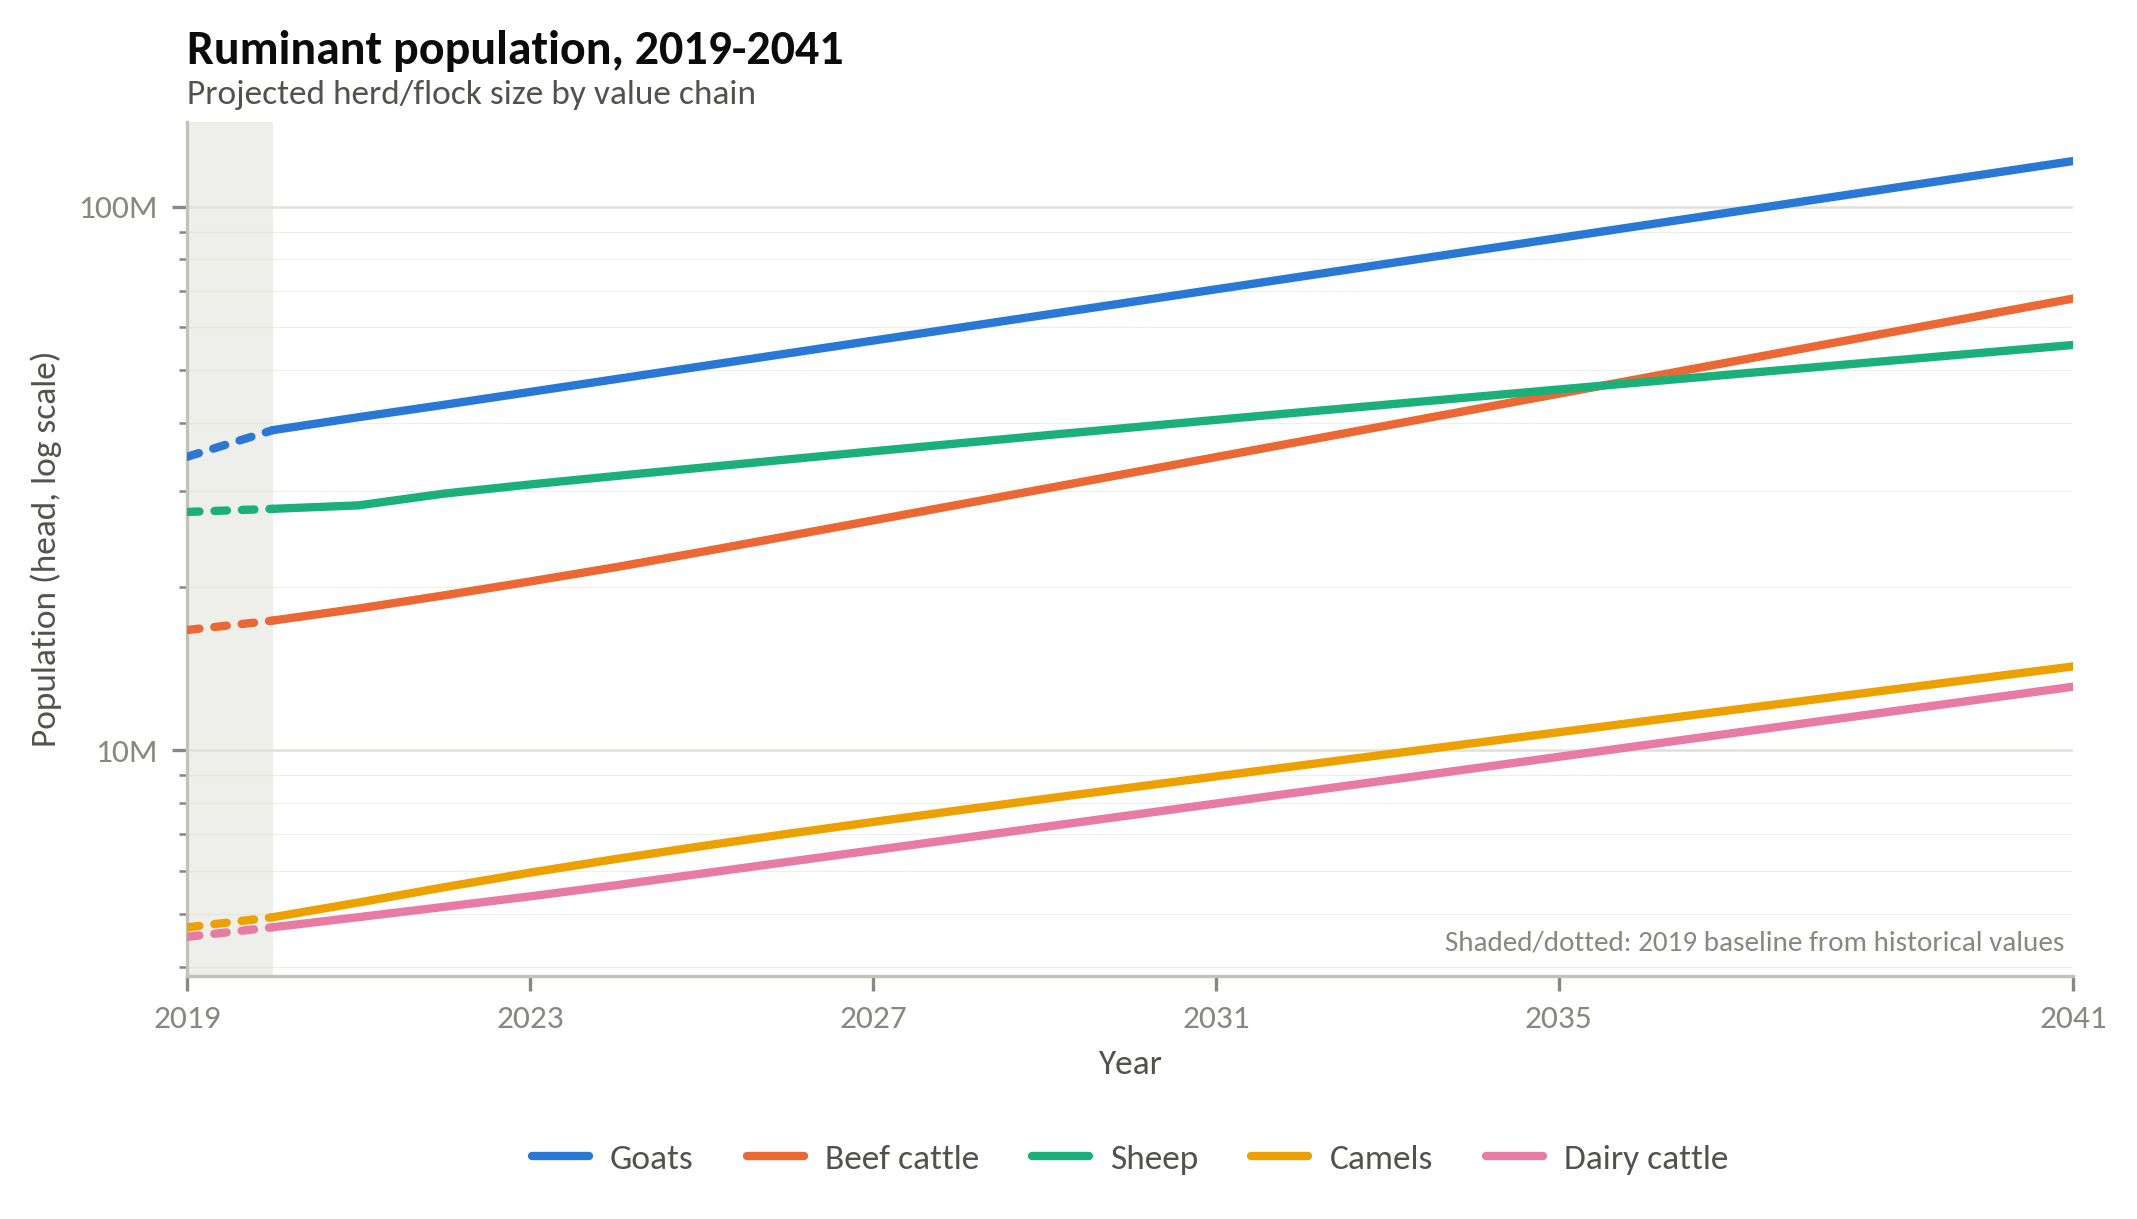
\includegraphics[width=\textwidth]{ruminant_pop.png}
\caption{Projected ruminant population by value chain, 2019--2041. Logarithmic vertical axis; the shaded band and dotted segment mark the 2019 baseline, which is a historical value.}
\label{fig:rumpop}
\end{figure}

\subsubsection{Non-ruminants}

Non-ruminant numbers grow far more slowly, from 106.3 million head in 2019 to
159.1 million in 2041, a 1.5-fold increase at 1.8\,\% per year
(Table~\ref{tab:nrpop}, Figure~\ref{fig:nrpop}). The aggregate conceals a divergence between the commercial and non-commercial segments of the poultry
chain. Layers and broilers expand by only about
10\,\% over 22 years (0.4\,\% per year) and plateauing after the early 2030s,
whereas indigenous poultry grow steadily at 3.0\,\% per year to 89.3 million
birds. The composition of the poultry flock shifts accordingly: indigenous birds
rise from 44.1\,\% to 58.1\,\% of total poultry, while the combined layer and
broiler share of all non-ruminants falls from 55.2\,\% to 40.5\,\%. The smallest
chains grow fastest: rabbits 4.4-fold at 7.0\,\% per year and pigs 3.5-fold at
5.9\,\% per year. Both start below one million head, so they remain marginal in
absolute terms. Managed bee colonies increase 2.7-fold to 3.5 million.

\begin{table}[htbp]
\centering
\caption{Non-ruminant population, 2019--2041 (thousands). Bee colonies are reported separately and excluded from the total.}
\label{tab:nrpop}
\small
\begin{tabular}{lrrrrrr}
\toprule
\textbf{Series} (\,000) & \textbf{2019} & \textbf{2025} & \textbf{2030} & \textbf{2035} & \textbf{2041} & \textbf{CAGR 2019--41 (\%)} \\
\midrule
Indigenous poultry & 46\,293 & 54\,774 & 65\,960 & 75\,970 & 89\,288 & 3.0 \\
Broilers & 45\,838 & 47\,477 & 49\,975 & 50\,175 & 50\,386 & 0.4 \\
Layers & 12\,844 & 13\,114 & 13\,946 & 14\,030 & 14\,089 & 0.4 \\
Rabbits & 737 & 1\,149 & 1\,585 & 2\,191 & 3\,235 & 7.0 \\
Pigs & 596 & 817 & 1\,097 & 1\,471 & 2\,088 & 5.9 \\
\textbf{Total (excl.\ colonies)} & 106\,309 & 117\,331 & 132\,563 & 143\,837 & 159\,086 & 1.8 \\
Bee colonies & 1\,289 & 1\,838 & 2\,384 & 2\,926 & 3\,489 & 4.6 \\
\bottomrule
\end{tabular}
\end{table}

\begin{figure}[htbp]
\centering
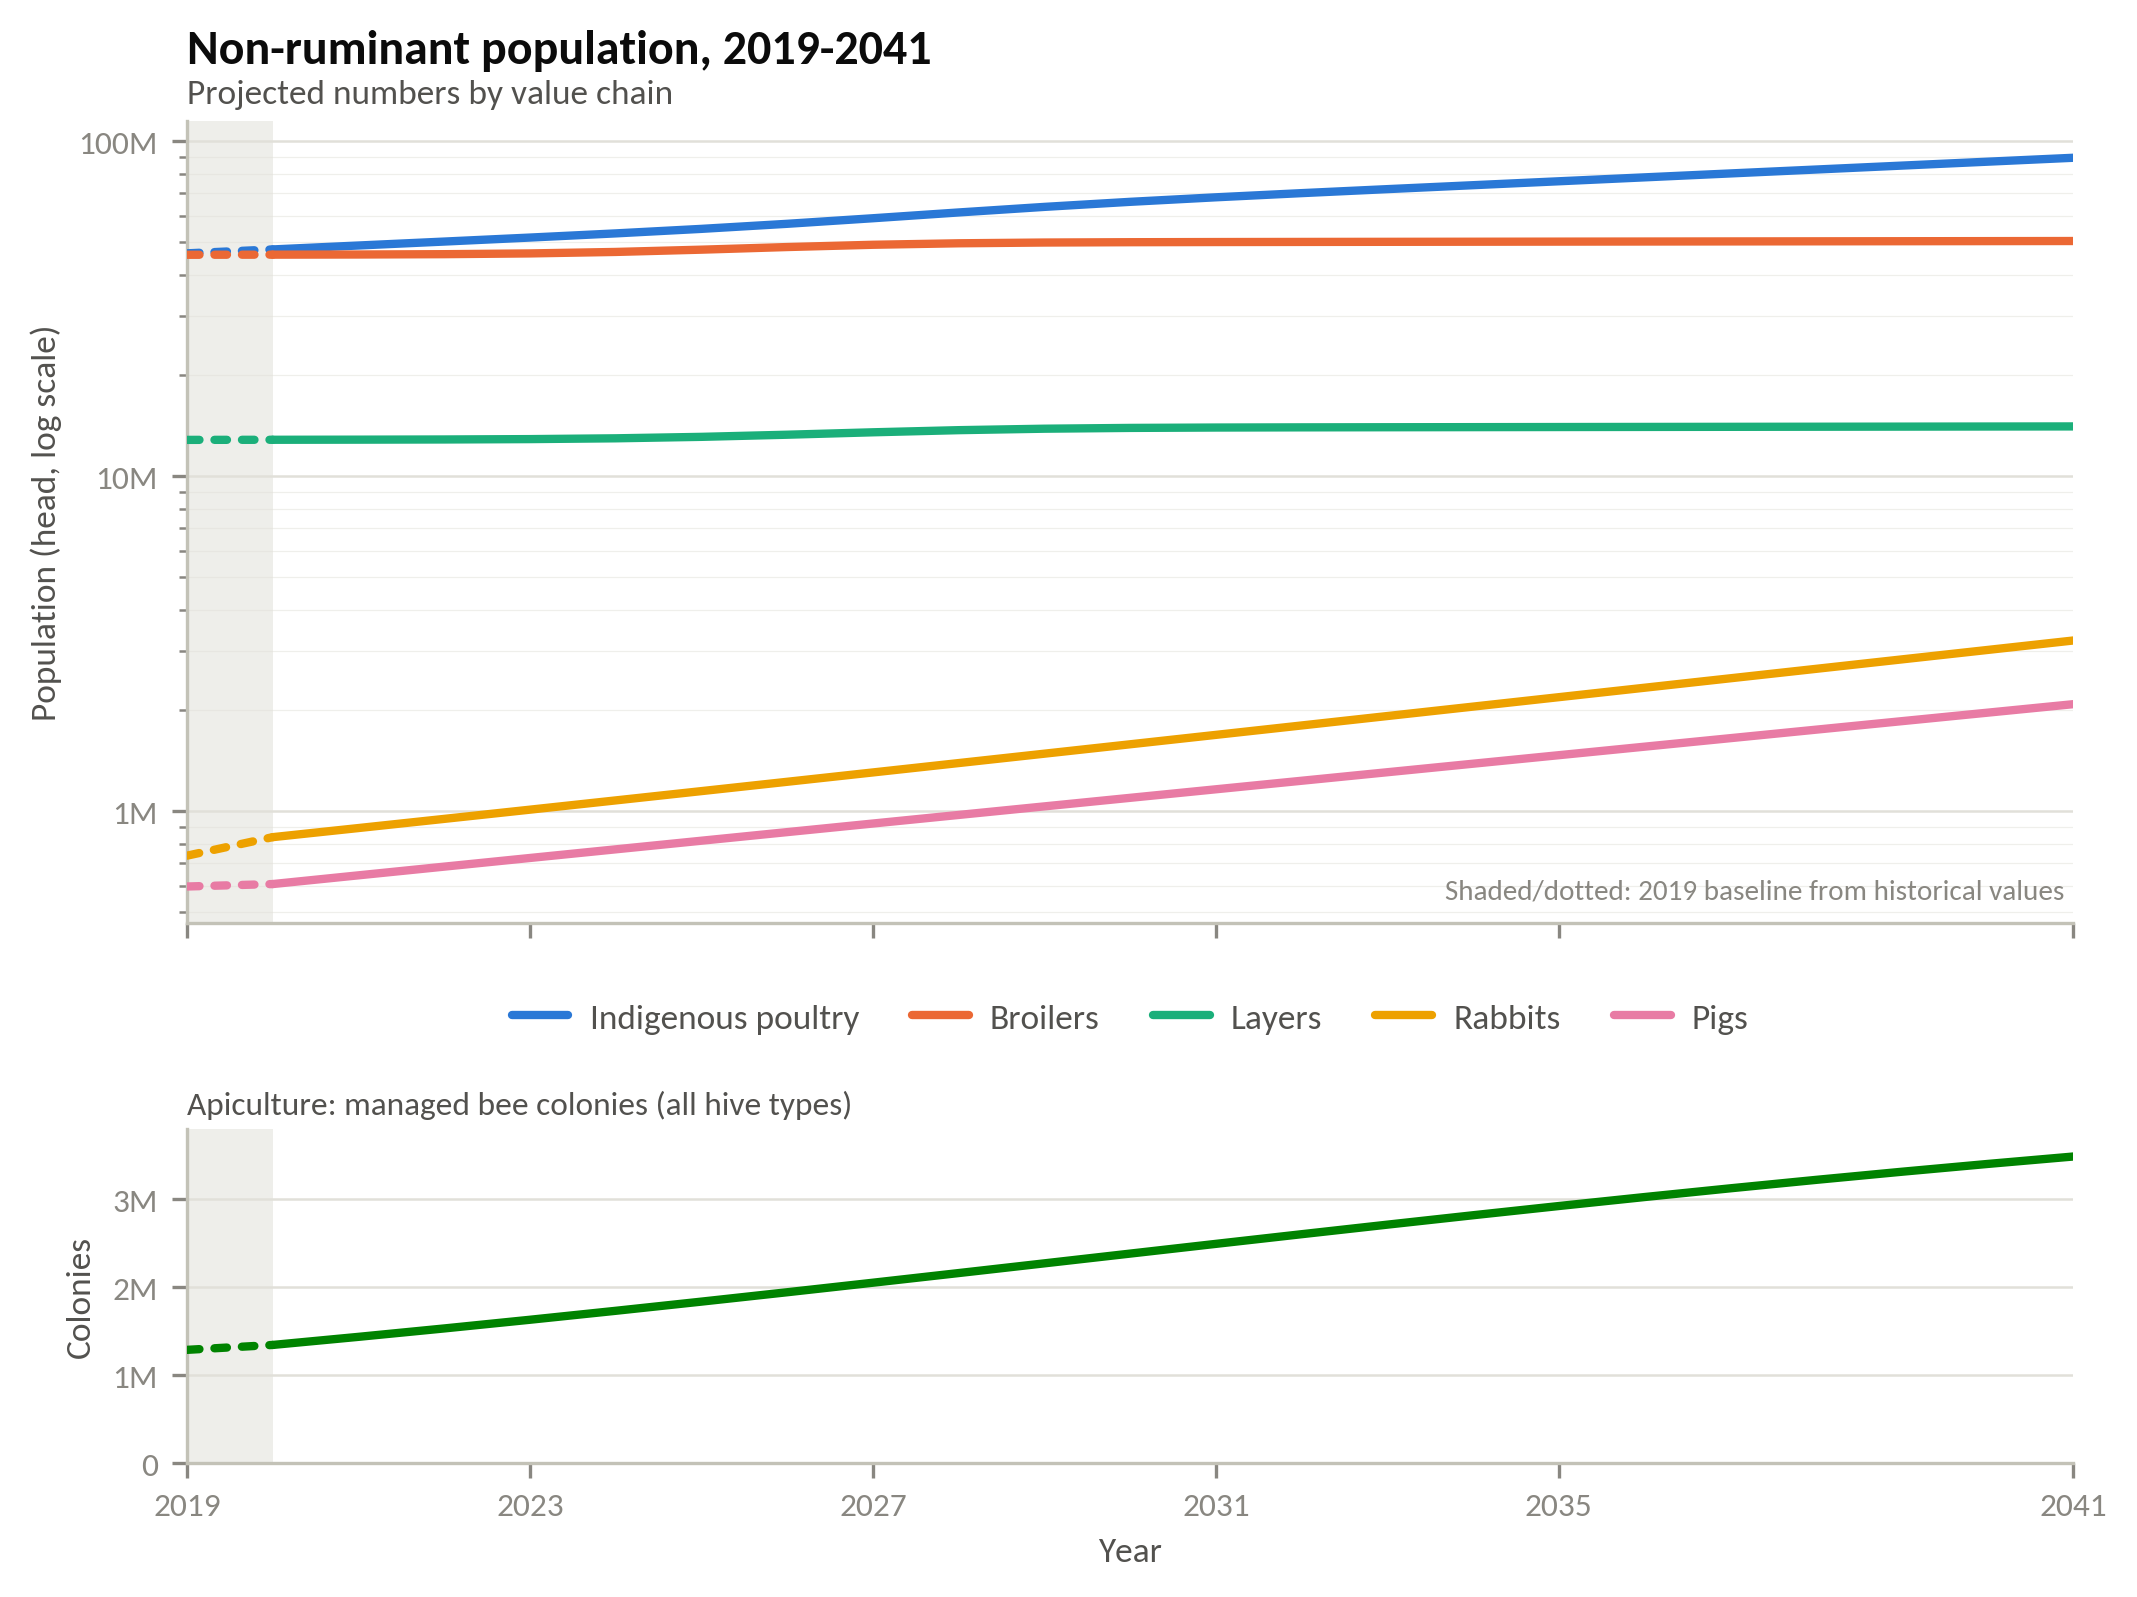
\includegraphics[width=\textwidth]{nonrum_pop.png}
\caption{Projected non-ruminant population by value chain, 2019--2041. Upper panel: livestock numbers (logarithmic axis). Lower panel: managed bee colonies (linear axis). Shaded bands and dotted segments mark the 2019 baseline, which is a historical value.}
\label{fig:nrpop}
\end{figure}

\subsection{Production}

\subsubsection{Ruminants}

Ruminant output expands across every product line (Table~\ref{tab:rumprod},
Figure~\ref{fig:rumprod}). Ten of the reported series carry a
step between the 2019 historical value and the 2020 projection
(Section~\ref{sec:dq}); for those series growth is described here from 2020, and
the 2019--2041 CAGRs in Table~\ref{tab:rumprod} should be read with that caveat.

Total milk from cattle, camels, and goats rises from 5.36 billion kg in 2020 to
15.41 billion kg in 2041, 5.2\,\% per year. Cattle milk remains the largest
single product at 9.26 billion kg in 2041; camel milk is the second largest at
5.61 billion kg, and since the two grow at almost identical rates from 2020
(5.0\,\% and 5.3\,\% per year) their ratio is close to stable, narrowing only
from 1.75:1 to 1.65:1. Goat milk is the fastest-growing dairy product at
6.6\,\% per year but remains a lot less at 531 million kg.

Meat output is led by chevon, which overtakes beef in 2020 and reaches 1.71
billion kg by 2041 against 1.37 billion kg of beef; both grow at 5.3--5.5\,\%
per year from 2020. Camel meat is the fastest-growing ruminant meat at 6.8\,\%
per year, though at 235 million kg in 2041 it remains well behind the two
leading products. Mutton grows slowest of all ruminant products at 1.2\,\% per
year from 2020, reaching 165 million kg, so the sheep chain contributes a
declining share of ruminant meat. Wool, the only product in the third group,
reaches 3.9 million kg at 2.8\,\% per year.

\begin{table}[htbp]
\centering
\caption{Ruminant production, 2019--2041 (million kg)}
\label{tab:rumprod}
\small
\begin{tabular}{lrrrrrr}
\toprule
\textbf{Series} (million kg) & \textbf{2019} & \textbf{2025} & \textbf{2030} & \textbf{2035} & \textbf{2041} & \textbf{CAGR 2019--41 (\%)} \\
\midrule
Cattle milk & 3\,087 & 4\,205 & 5\,375 & 6\,883 & 9\,263 & 5.1 \\
Camel milk & 985 & 2\,672 & 3\,369 & 4\,248 & 5\,611 & 8.2 \\
Goat milk & 156 & 222 & 292 & 383 & 531 & 5.7 \\
Chevon & 53.9 & 718 & 942 & 1\,236 & 1\,712 & 17.0 \\
Beef & 322 & 479 & 656 & 919 & 1\,375 & 6.8 \\
Camel meat & 57.6 & 104 & 139 & 178 & 235 & 6.6 \\
Mutton & 49.4 & 100 & 117 & 137 & 165 & 5.6 \\
Wool & 0.84 & 2.40 & 2.80 & 3.26 & 3.92 & 7.3 \\
\bottomrule
\end{tabular}
\end{table}

\begin{figure}[htbp]
\centering
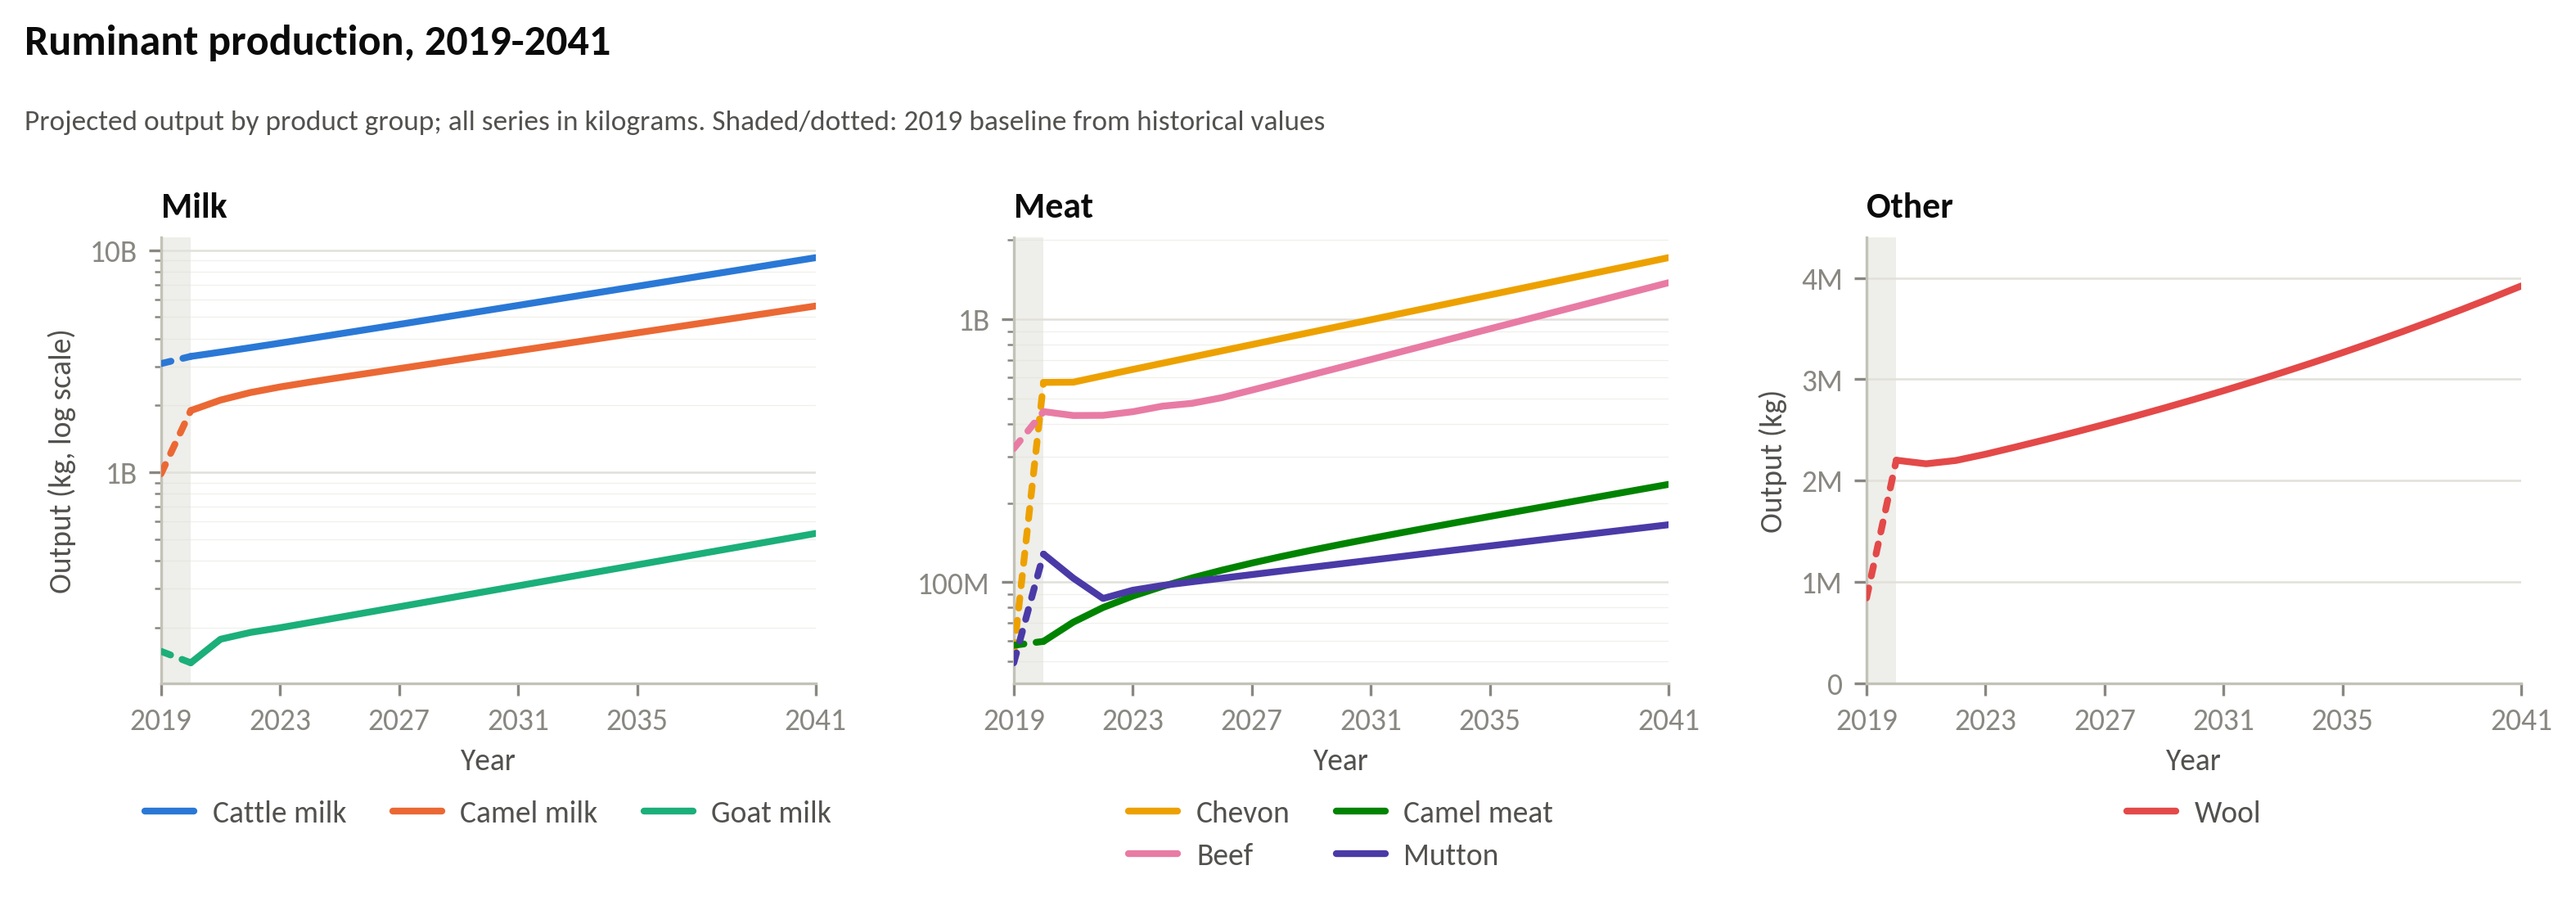
\includegraphics[width=\textwidth]{ruminant_prod.png}
\caption{Projected ruminant production, 2019--2041, by product group: milk, meat, and wool. Milk and meat panels use logarithmic vertical axes; the wool panel is linear. Shaded bands and dotted segments mark the 2019 baseline, which is a historical value.}
\label{fig:rumprod}
\end{figure}

\subsubsection{Non-ruminants}

Non-ruminant production growth is more subdued and closely tracks the population
trajectories (Table~\ref{tab:nrprod}, Figure~\ref{fig:nrprod}). Poultry meat,
the largest non-ruminant product, grows only 1.3\,\% per year to 109.7 million
kg, consistent with the plateau in commercial bird numbers. Pork grows at
4.0\,\% per year to 34.1 million kg and rabbit meat at 4.6\,\% per year (from
2020) to 4.2 million kg. The apiculture products grow fastest: honey at 5.1\,\%
per year to 41.6 million kg and beeswax at 5.4\,\% per year (from 2020) to 6.5
million kg. Honey output exceeds pork output in absolute mass from 2021 onward
and is 1.2 times pork by 2041, making apiculture the second-largest
non-ruminant product group by mass. Egg production, reported in trays and
therefore shown in its own panel on a linear axis, rises from 180.4 million
trays in 2020 to 228.7 million in 2041 (1.1\,\% per year); the 501.3 million
trays recorded for 2019 is inconsistent with the remainder of the series.

\begin{table}[htbp]
\centering
\caption{Non-ruminant production, 2019--2041 (million kg; eggs in million trays)}
\label{tab:nrprod}
\small
\begin{tabular}{lrrrrrr}
\toprule
\textbf{Series} (million) & \textbf{2019} & \textbf{2025} & \textbf{2030} & \textbf{2035} & \textbf{2041} & \textbf{CAGR 2019--41 (\%)} \\
\midrule
Poultry meat & 82.4 & 88.8 & 97.6 & 103 & 110 & 1.3 \\
Pork & 14.4 & 18.2 & 22.2 & 27.0 & 34.1 & 4.0 \\
Rabbit meat & 1.76 & 2.03 & 2.55 & 3.19 & 4.18 & 4.0 \\
Honey & 13.9 & 22.4 & 29.2 & 35.4 & 41.6 & 5.1 \\
Beeswax & 1.37 & 3.39 & 4.48 & 5.50 & 6.54 & 7.4 \\
Eggs (million trays) & 501 & 189 & 208 & 217 & 229 & -3.5 \\
\bottomrule
\end{tabular}
\end{table}

\begin{figure}[htbp]
\centering
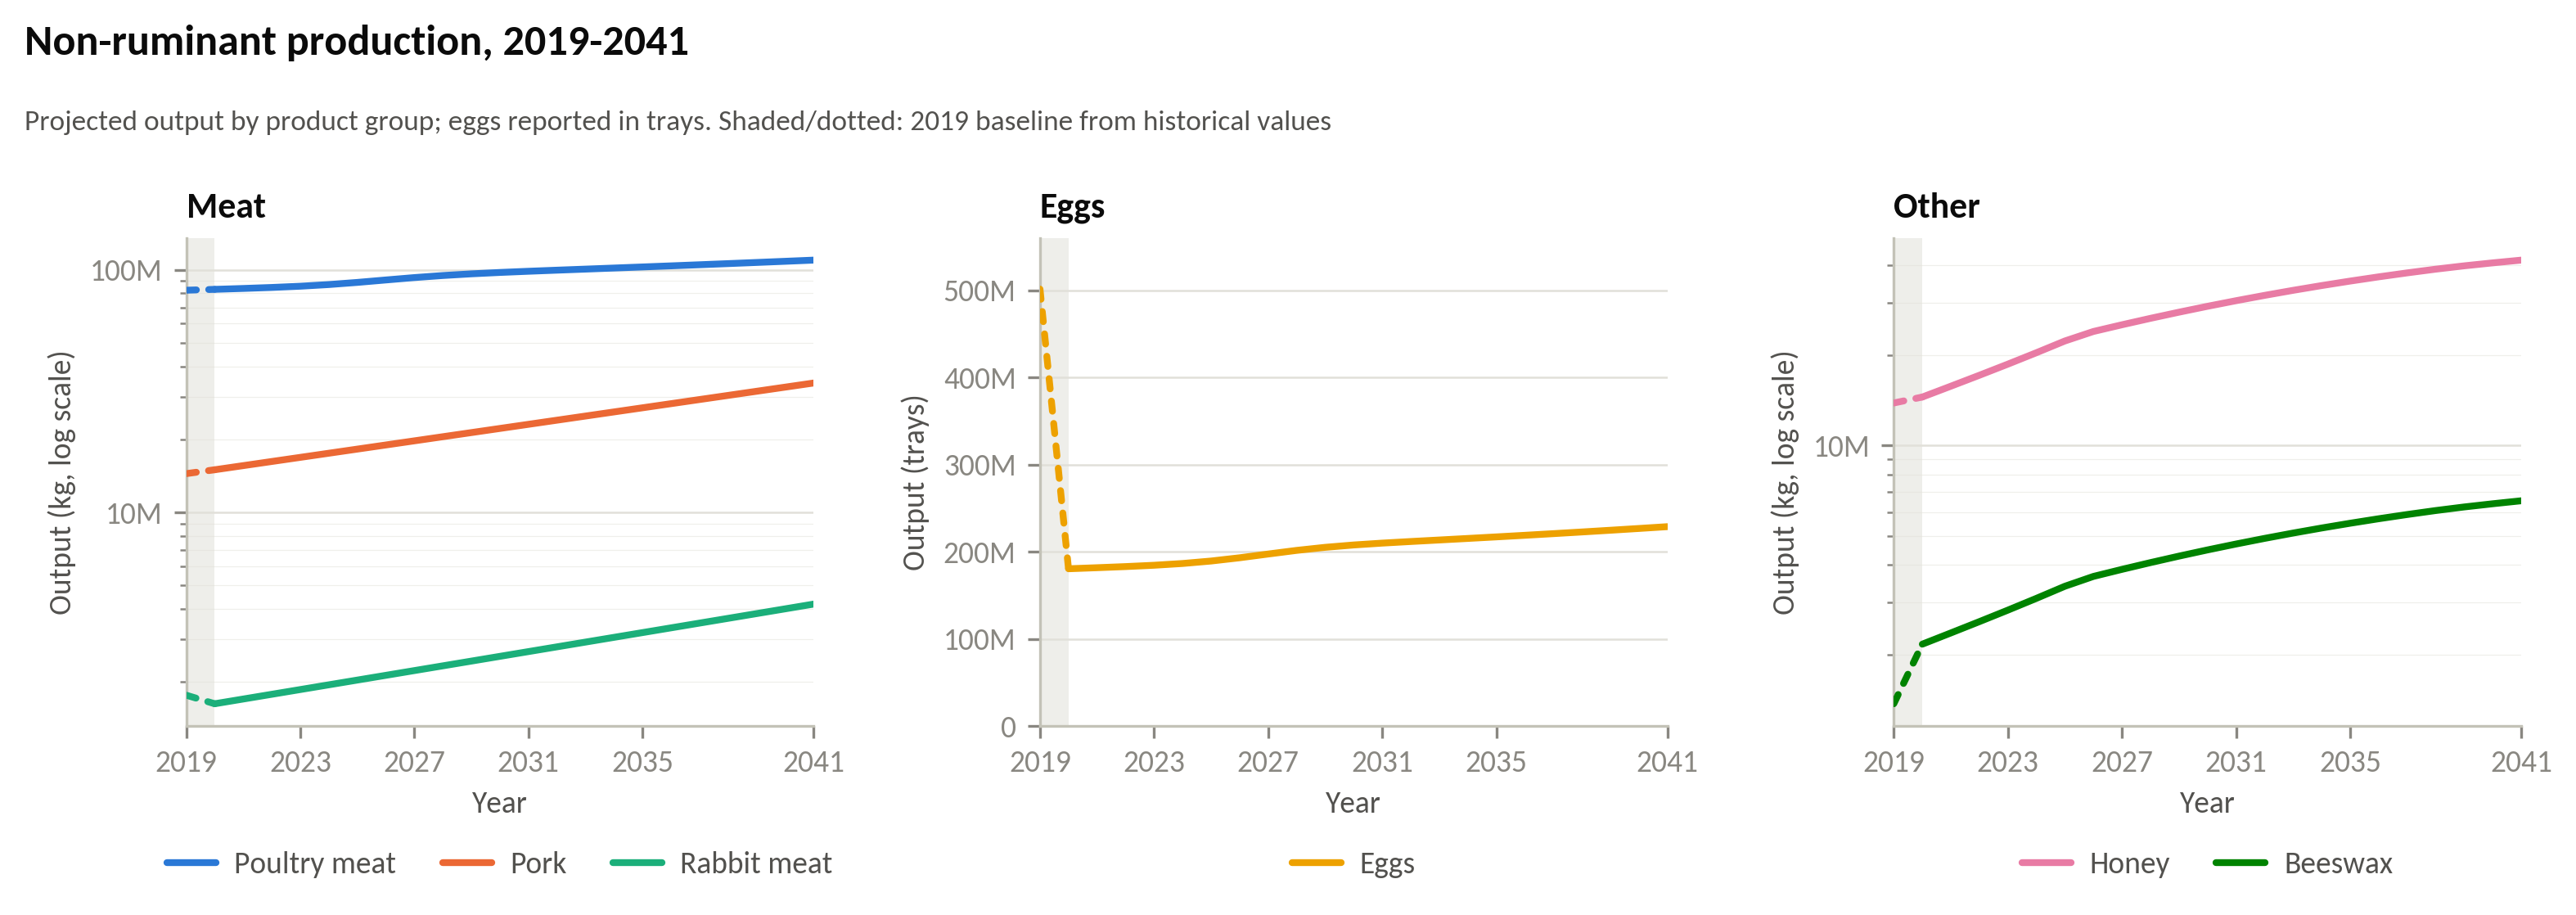
\includegraphics[width=\textwidth]{nonrum_prod.png}
\caption{Projected non-ruminant production, 2019--2041, by product group: meat, eggs, and apiculture products. Meat and other panels use logarithmic vertical axes; the egg panel is linear because eggs are reported in trays. Shaded bands and dotted segments mark the 2019 baseline, which is a historical value.}
\label{fig:nrprod}
\end{figure}

\subsection{Feed demand}

\subsubsection{Ruminants}

Ruminant chains account for the great majority of projected feed demand
(Table~\ref{tab:rumfeed}, Figure~\ref{fig:rumfeed}). Total requirement rises
from 105.8 million tonnes DM in 2020 to 353.8 million tonnes in 2041, 5.9\,\%
per year. Beef cattle alone account for 58.8 million tonnes in 2020 and 218.3
million in 2041, more than the other four ruminant chains combined in every year
of the period. Their share rises from 55.5\,\% to 61.7\,\% as they grow at
6.4\,\% per year, the fastest of the five chains. Goats follow at 6.1\,\% per
year to 36.2 million tonnes and camels at 5.6\,\% to 42.2 million tonnes, the
latter overtaking dairy cattle in 2023; dairy cattle reach 41.2 million tonnes
at 4.9\,\% per year. Sheep demand grows slowest, from 8.0 to 15.9 million
tonnes at 3.3\,\% per year.

\begin{table}[htbp]
\centering
\caption{Ruminant feed demand, 2020--2041 (thousand tonnes DM)}
\label{tab:rumfeed}
\small
\begin{tabular}{lrrrrrr}
\toprule
\textbf{Series} (\,000 t DM) & \textbf{2020} & \textbf{2025} & \textbf{2030} & \textbf{2035} & \textbf{2041} & \textbf{CAGR 2020--41 (\%)} \\
\midrule
Beef cattle & 58\,791 & 74\,615 & 104\,258 & 145\,888 & 218\,333 & 6.4 \\
Camels & 13\,474 & 19\,399 & 25\,167 & 31\,904 & 42\,184 & 5.6 \\
Dairy cattle & 15\,064 & 18\,646 & 23\,877 & 30\,584 & 41\,165 & 4.9 \\
Goats & 10\,528 & 15\,187 & 19\,929 & 26\,151 & 36\,233 & 6.1 \\
Sheep & 7\,989 & 9\,332 & 11\,135 & 13\,133 & 15\,889 & 3.3 \\
\textbf{Total ruminants} & 105\,846 & 137\,177 & 184\,366 & 247\,660 & 353\,805 & 5.9 \\
\bottomrule
\end{tabular}
\end{table}

\begin{figure}[htbp]
\centering
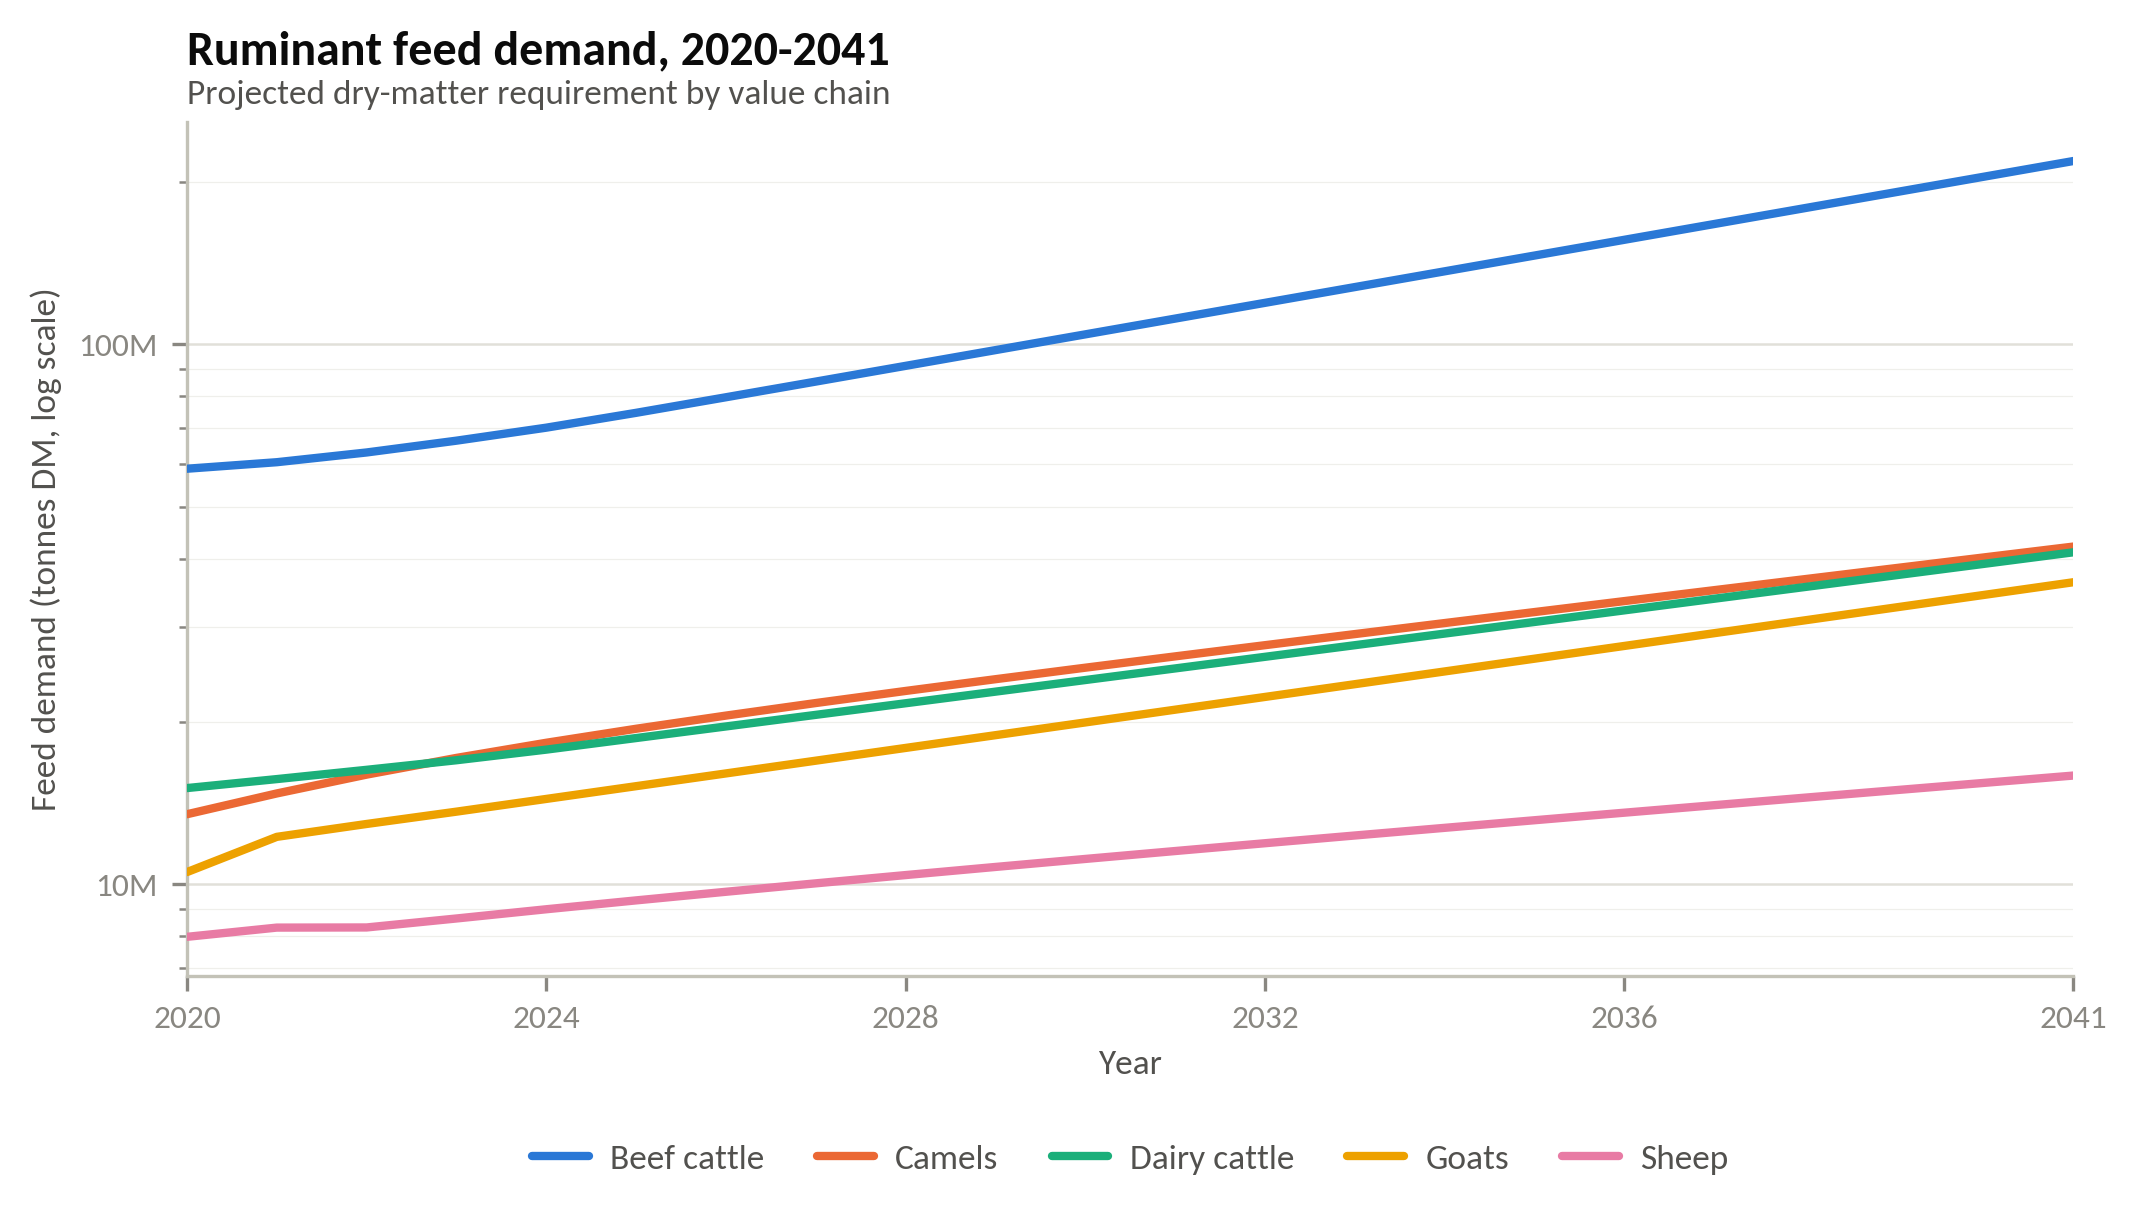
\includegraphics[width=\textwidth]{ruminant_feed.png}
\caption{Projected ruminant dry-matter feed demand by value chain, 2020--2041. Logarithmic vertical axis. (Section~\ref{sec:dq}).}
\label{fig:rumfeed}
\end{figure}

\subsubsection{Non-ruminants}

Non-ruminant feed demand is less, rising from
3.29 million tonnes in 2020 to 6.46 million tonnes in 2041 at 3.3\,\% per year
(Table~\ref{tab:nrfeed}, Figure~\ref{fig:nrfeed}). That is 1.8\,\% of the
ruminant total in 2041. Poultry accounts for the largest share throughout but grows
slowest at 1.9\,\% per year to 2.83 million tonnes, so its share falls from
57.7\,\% to 43.8\,\%. Apiculture nectar demand grows at 5.0\,\% per year to 2.49
million tonnes, reaching 88\,\% of poultry feed demand by 2041. Pig feed demand
reaches 1.09 million tonnes (4.1\,\% per year) and rabbit demand 52.7 thousand
tonnes (4.5\,\% per year).

\begin{table}[htbp]
\centering
\caption{Non-ruminant feed demand, 2020--2041 (thousand tonnes)}
\label{tab:nrfeed}
\small
\begin{tabular}{lrrrrrr}
\toprule
\textbf{Series} (\,000 t) & \textbf{2020} & \textbf{2025} & \textbf{2030} & \textbf{2035} & \textbf{2041} & \textbf{CAGR 2020--41 (\%)} \\
\midrule
Poultry & 1\,900 & 2\,067 & 2\,350 & 2\,556 & 2\,828 & 1.9 \\
Apiculture (nectar) & 900 & 1\,259 & 1\,706 & 2\,093 & 2\,489 & 5.0 \\
Pigs & 473 & 579 & 707 & 862 & 1\,092 & 4.1 \\
Rabbits & 20.9 & 25.8 & 32.2 & 40.3 & 52.7 & 4.5 \\
\textbf{Total non-ruminants} & 3\,293 & 3\,931 & 4\,795 & 5\,552 & 6\,462 & 3.3 \\
\bottomrule
\end{tabular}
\end{table}

\begin{figure}[htbp]
\centering
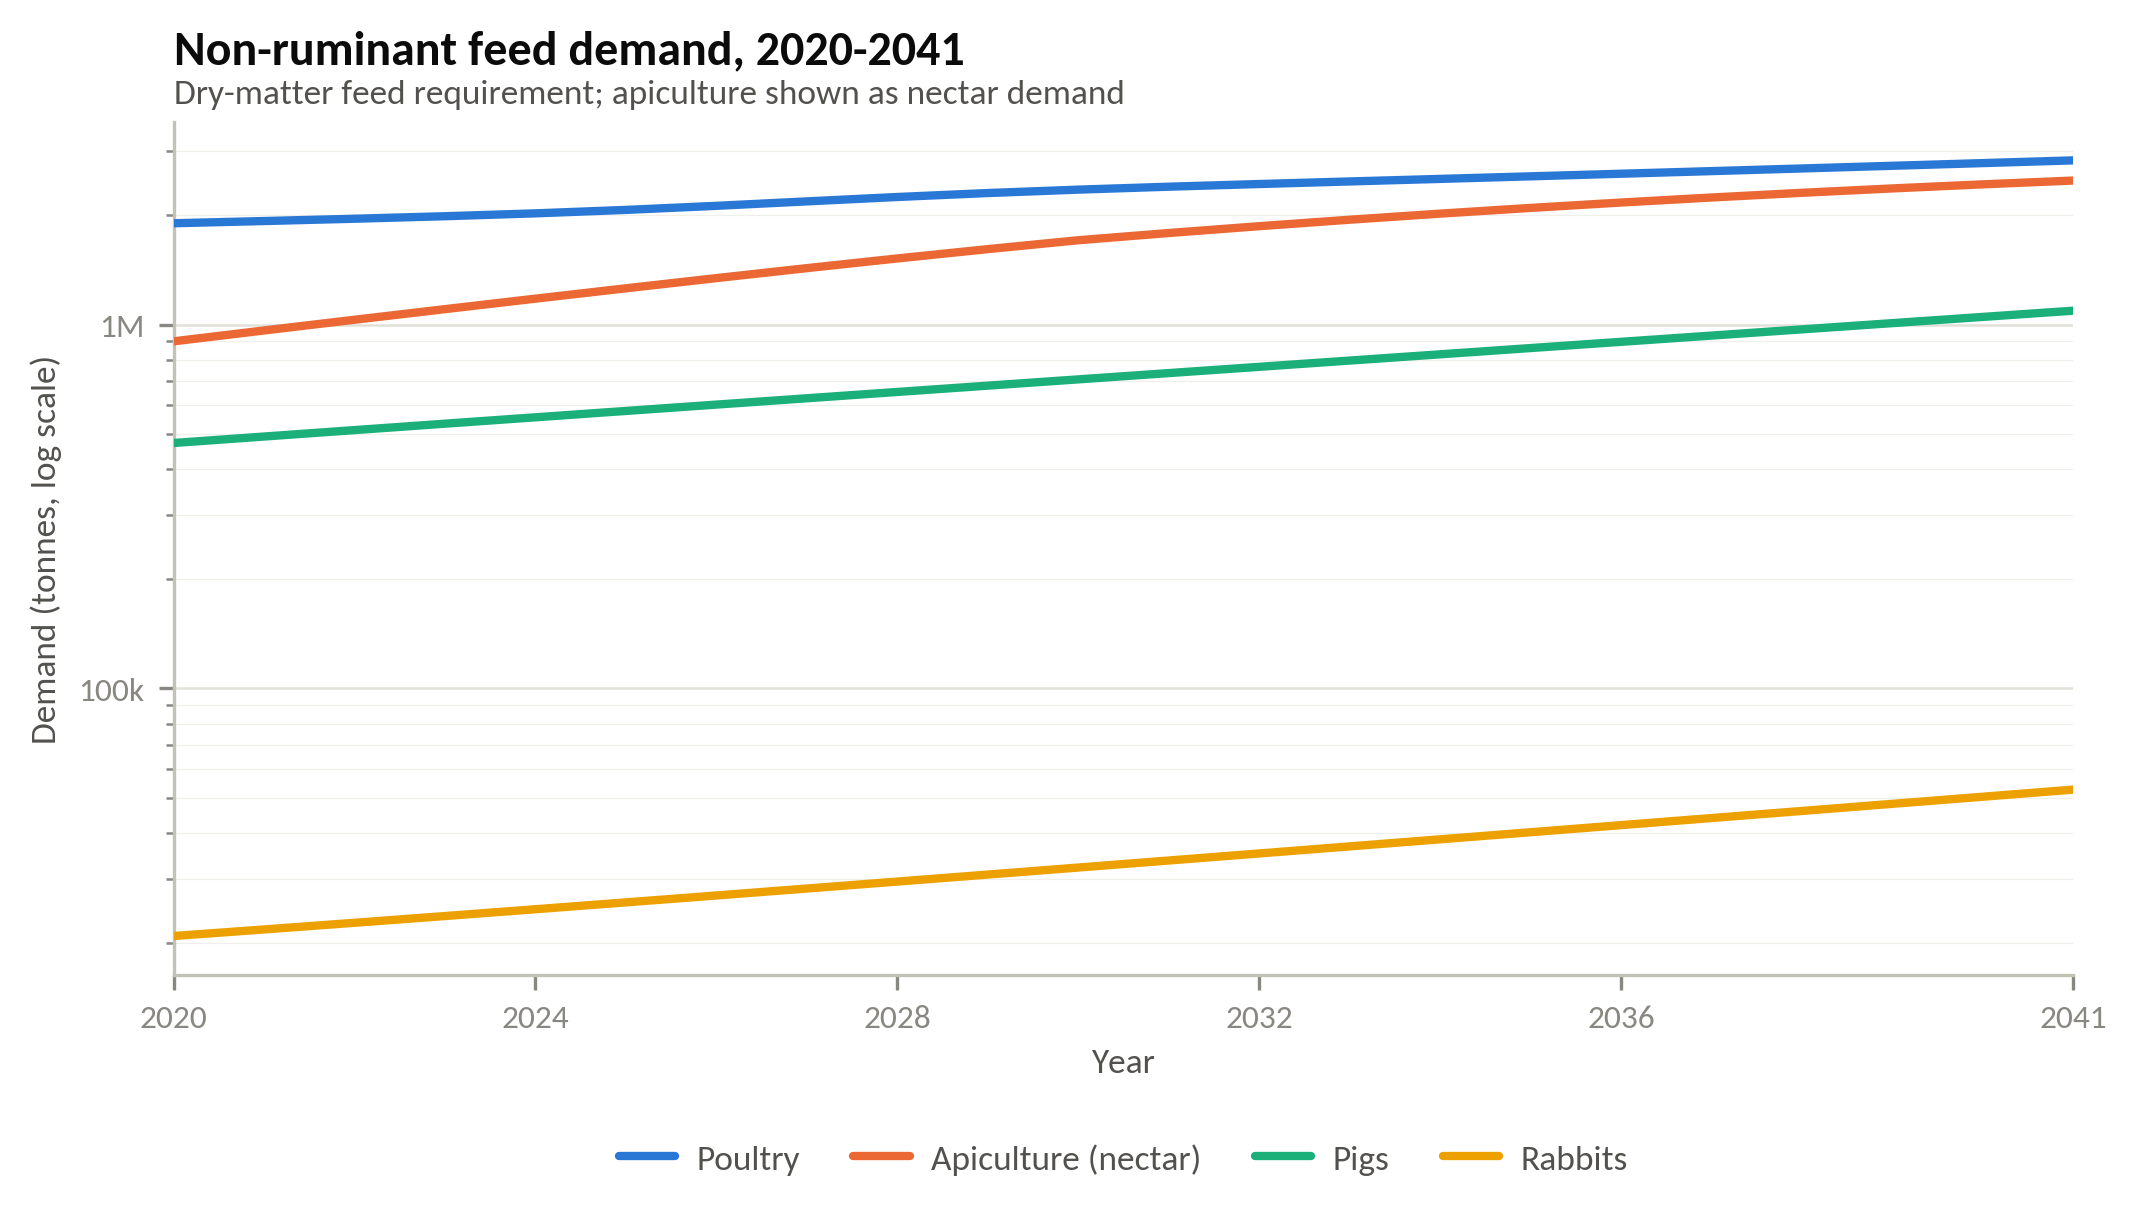
\includegraphics[width=\textwidth]{nonrum_feed.png}
\caption{Projected non-ruminant feed demand by value chain, 2020--2041. Apiculture is shown as nectar demand. Logarithmic vertical axis.}
\label{fig:nrfeed}
\end{figure}